%%%%%%%%%%%%%%%%%%%%%%%%%%%%%%%%%%%%%%%%%%%%%%%%%%%%%%%%%%%%%%%%%%%%%%%%%%%%%%%%
%2345678901234567890123456789012345678901234567890123456789012345678901234567890
%        1         2         3         4         5         6         7         8
\documentclass[letterpaper, 10 pt, conference]{ieeeconf}  % Comment this line out if you need a4paper
\IEEEoverridecommandlockouts                              % This command is only needed if 
                                                         % you want to use the \thanks command
\usepackage[utf8]{inputenc}
\usepackage{amsmath}
\usepackage{bm}
\usepackage{amssymb}
\usepackage{graphicx}
\usepackage{booktabs}
\usepackage{mathrsfs}
\usepackage{amsbsy}
\usepackage{caption}
\usepackage{float}
\usepackage{subcaption}
\usepackage{varwidth}
\usepackage{algorithm}
\usepackage{tabularx}
\usepackage{yhmath}
\usepackage{multirow}
\usepackage{multicol}
\usepackage{booktabs}
\usepackage{rotating}
\usepackage[table]{xcolor}
\definecolor{grey}{rgb}{0.9,0.9,0.9}
\usepackage[noend]{algpseudocode}
\usepackage[top=60pt,left=48pt,right=48pt,bottom=45pt]{geometry}	
\usepackage{dsfont}
\usepackage{environ}
\usepackage[framemethod=TikZ]{mdframed}
\usepackage{algorithm}
\usepackage{accents}\newcommand\addtag{\refstepcounter{equation}\tag{\theequation}}
\usepackage{etoolbox}
\usepackage{graphicx}
\usepackage{rotating}
\usepackage{enumerate}
\usepackage[colorlinks]{hyperref}
\usepackage{relsize}
\usepackage{gensymb}
\usepackage{cleveref}
\usepackage{threeparttable}
\usepackage{xspace} 
\usepackage{colortbl}
\definecolor{Gray}{gray}{0.9}
\newcommand{\comFB}[1]{\noindent\colorbox{yellow}{\parbox{\dimexpr\columnwidth-1\fboxsep}{[FB: #1]}}}
%%% Customized commands
%%% math commands
\newcommand{\mvec}[1]{\bm{#1}}
\newcommand{\dmvec}[1]{\dot{\mvec{{#1}}}}
\newcommand{\ddmvec}[1]{\ddot{\mvec{{#1}}}}

\newcommand{\xt}{\mvec{x}(t)}
\newcommand{\ut}{\mvec{u}(t)}

\newcommand{\st}{\text{s.t.}}
\newcommand{\g}{\mvec{g}}
\newcommand{\q}{\mvec{q}}
\newcommand{\dq}{\dmvec{q}}
\newcommand{\ddq}{\ddmvec{q}} 

%%% table commands
\newcommand{\mymultirow}[2]{\parbox[t]{2mm}{\multirow{#1}{*}{\rotatebox[origin=c]{90}{#2}}}}
%%% Document
\title{\LARGE \bf Bioptim, a Python interface for Musculoskeletal Optimal Control in Biomechanics}
\author{author$\#1$\textsuperscript{a,*}, author$\#2$\textsuperscript{a}, author$\#3$\textsuperscript{b}  and  author$\#4$\textsuperscript{a}% <-this % stops a space
\thanks{\textsuperscript{a}\,Laboratoire de Simulation et Modélisation du Mouvement, Faculté de Médecine, Université de Montréal, Laval, QC, Canada}%
\thanks{\textsuperscript{b}\,other, elsewhere}%
\thanks{\textsuperscript{*}\,author$\#1$@umontreal.ca}
}

%%% User commands

\usepackage{pdfrender}
\DeclareRobustCommand*{\pmbb}[1]{%
  \textpdfrender{
    TextRenderingMode=Stroke,
    LineWidth=.1pt,
  }{#1}%
}
\NewEnviron{comeq}{%
\par\vspace{0ex}
\begin{mdframed}[outerlinewidth=0.5,leftmargin=10,rightmargin=-10pt,backgroundcolor=white,hidealllines=true,leftline=true,
innertopmargin=0pt,splittopskip=0, skipbelow=\baselineskip, innerbottommargin=0pt%
skipabove=0ex]%
\vspace{-0ex}\hspace{0pt}\textit{Proof:}%
\itshape
\begin{equation*} 
\begin{split}
\BODY
\end{split}
\end{equation*}
\end{mdframed}
}
\newcommand{\pd}[2]{\frac{\partial #1}{\partial #2}}
\def\abs{\operatorname{abs}}
\def\argmax{\operatornamewithlimits{arg\,max}}
\def\argmin{\operatornamewithlimits{arg\,min}}
\def\diag{\operatorname{Diag}}
\newcommand{\eqRef}[1]{(\ref{#1})}
\newcommand{\dbtilde}[1]{\accentset{\approx}{#1}}
\newcommand{\state}{\mathbf{x}}
\newcommand{\dstate}{\dot{\mathbf{x}}}
\newcommand{\control}{\mathbf{u}}
\newcommand{\param}{\mathbf{p}}
\newcommand{\bioptim}{\textit{Bioptim}\xspace}



\hyphenpenalty=10000

\begin{document}

\maketitle
\thispagestyle{plain}
\pagestyle{plain}

\begin{abstract}
The abstract
\end{abstract}

\textbf{Keywords -- TODO}



\section{Introduction}\label{sec:introduction}
Biomechanics researchers rely on numerical simulations of motion to gain understanding on a variety of scientific topics such as the physiological causes of movement disorders and their consequences on health \cite{pizzolato2015ceinms}, the estimation of non-measurable physiological quantities (e.g., muscle forces \cite{bailly2020real}) and the optimality of human movement \cite{porsa2016direct}.
The musculoskeletal models used in these simulations generally have a large number of degrees of freedom and they are governed by several ordinary differential equations (ODEs) which mainly describe multibody and muscle activation dynamics.
The complexity of these systems has led scientists to formulate their simulations as optimal control problems (OCP), relying on efficient non-linear optimization software to find trajectories that fulfill a desired task while enforcing the system dynamics and minimizing a cost (e.g. motion duration, energy expenditure, matching experimental data, etc.).
Up to very recently, there was no off-the-shelf software available to the community to quickly formulate and solve such musculoskeletal OCPs \cite{Charles2013}. 
Consequently, researchers had to develop their own solutions, with little or no dissemination to the community, limiting  synergies between researchers.


As a result, many approaches coexist to formulate and solve OCPs in the biomechanical literature. 
The formulation, also called discretization, consists in turning a continuous trajectory optimization problem into a generic discrete non-linear program (NLP) that is solved using a dedicated algorithm. 
The main family of so-called \textit{direct} transcription methods comes from numerical optimal control. 
They consist in straightforwardly choosing the state and/or the control as optimization variables at a given number of points along the trajectory and they rely on the integration of the system dynamics between these points. 

For instance, the \textit{direct collocation} method has shown its efficiency in some studies investigating human motion \cite{febrer-nafriaComparisonDifferentOptimal2020, ezatiComparisonDirectCollocation2020}.
It consists in approximating the integration of the system dynamics using polynomials that describe the state and control trajectories.
Its main advantages are that it leads to very sparse NLPs, that knowledge about the state trajectory can be used in the initialization, and that it handles unstable systems well. 
Its major disadvantage is that adaptive integration error control implies regridding the whole problem and thus changes the NLP dimensions~\cite{diehl2006fast}.
\textit{Direct multiple shooting} is another direct method that was also applied with success in a lot of biomechanics \cite{koschorreck2012modeling, felis2013modeling, charbonneau2020optimal, bailly2020optimal} and robotics \cite{diehl2006fast, giftthaler2018control, bailly2018mechanical} studies.
Its advantages are mostly the same as for direct collocation in addition to combining integration error control with fixed NLP dimensions, as it relies on possibly adaptive ODE solvers to integrate the system dynamics.
Besides direct methods, other choices can be made, as in \cite{yeadon2000mechanics, begon2009effect}, where the optimization variables are instants at which a switch in the motor strategy occurs, using polynomials function (4th, 5th order) in-between, or in \cite{leboeuf2006energetic, huchez2015local}, where the optimization variables are the coefficients of fourth order polynomial approximations of the states, with linking conditions to enforce the continuity of the controls. 
These last approaches are less generic than the direct methods as they either require a prior knowledge about the state and control trajectories. 
Most of the time, when investigating complex biomechanics issues, we do not have this information. 

\begin{figure}[t!]
\centering
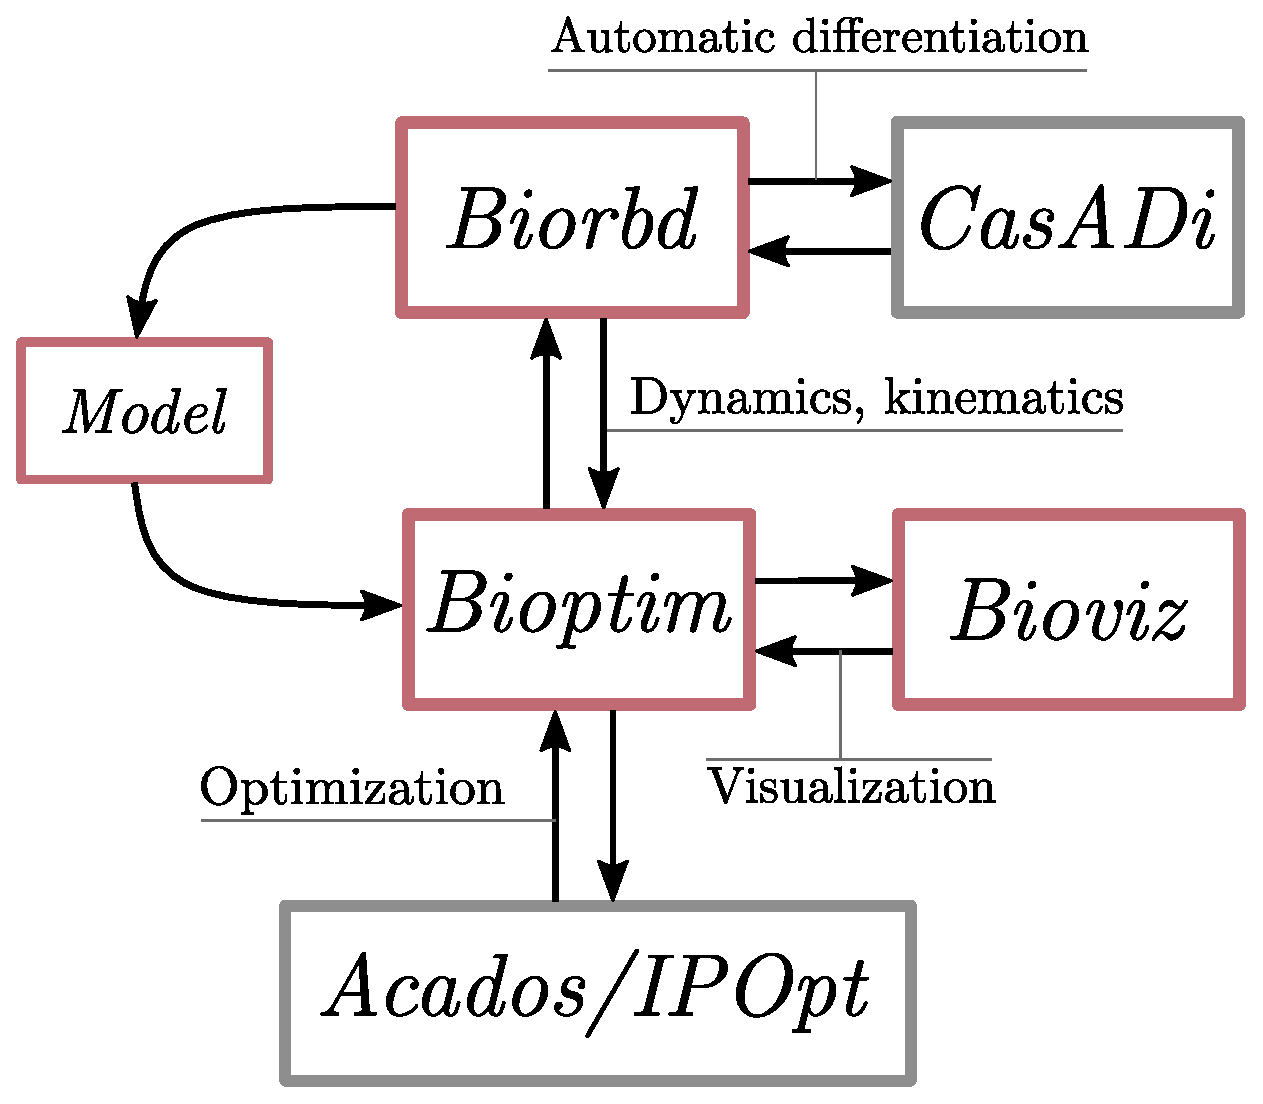
\includegraphics[width=0.9\columnwidth]{figures/dependencies.eps}
\caption{\bioptim dependencies flowchart. The red-boxed software are developed by the S2M team. The \bioptim part is further detailed in Fig.~\ref{fig:flowchart}.}
\label{fig:dependencies}
\vspace*{-0.8cm}
\end{figure}

Concerning the non-linear solver, a variety of software exist and have been used to solve transcribed musculoskeletal NLPs.
They can use different heuristics: interior point methods (\ipopt, \cite{wachter2006implementation}) or sequential quadratic programming (\textit{snopt} \cite{gill2005snopt}, \acados \cite{verschueren2018towards}), but they are all gradient based.
Therefore, derivatives of the NLP cost function and constraints are required to perform optimization.
These derivatives can be obtained by finite differences (often implemented but inaccurate thus comprising convergence) or computed exactly using automatic differentiation (requiring to write all dependencies of the software in symbolic variables), using, e.g., \casadi \cite{andersson2019casadi}.

In order to promote the use of musculoskeletal optimal control among biomechanics researcher, we identified a strong need for a dedicated tool, as shown by the recently launched \moco \cite{dembia2020opensim}. 
The biomechanics community being mainly composed of software users, such a tool should request a flexible user interface written in a widely used high-level and if possible open-source language (e.g. Python) with a low-level core (e.g. C++) for efficiency. 

To develop such a software, four interrelated components are essential in our opinion: \textit{i)} a musculoskeletal modeling software, with a visualization module (multibody kinematics and dynamics, muscle dynamics, etc.), \textit{ii)} a method for automatic differentiation, \textit{iii)} a discretization approach, and \textit{iv)} one or several nonlinear programming (NLP) solvers. 
General-purpose optimal control software (e.g. \gpopsii \cite{patterson2014gpops}, \muscodii \cite{leineweber2003efficient1,leineweber2003efficient2}, \acado \cite{houska2011acado}]) address \textit{ii)} to \textit{iv)} but they need to be interfaced with a musculoskeletal modeling module and they do not provide any built-in biomechanics features (physiological cost functions, kinematic constraints, etc.). 
In that sense, the aforementioned \moco, is a welcome initiative that draws its strength from its integration with the widely used \opensim.
However, it faces the following limitations: it uses finite differences to avoid the complexity of adapting the \opensim codebase to support automatic differentiation, it uses direct collocation as transcription method, preventing the use of adaptive ODE solvers and it is not as flexible as required by the community, since it requires the user to develop new features, such as new objective functions, in C++. 

The objective of the present paper is to introduce \bioptim\footnote{\url{https://github.com/pyomeca/bioptim}\\\comment{DOI: 10.5281/zenodo.4562883}{J'ai aussi mis la citation après, mais on peut la retirer..}}~\cite{bioptim2021michaud}, an \comment{open-source}{je l'ai corrigé quelques fois, mais ça semble revenir, open source ne prend pas de tiret} optimal control software dedicated to musculoskeletal biomechanics.
\bioptim is based on C++ code for computational efficiency but the user interface is written in Python for flexibility and ease-of-use. 
The OCP transcription uses direct multiple shooting to preserve the possibility of using arbitrarily accurate ODE solvers for the integration, which is fully parallelized for more efficiency.
\bioptim's core is fully written in \casadi symbolics to benefit from algorithmic differentiation and to exploit \casadi 's interface with several non-linear solvers (\ipopt, \snopt).
Moreover, \bioptim is interfaced with the cutting-edge solver \acados, a recent NLP solver dedicated to direct multiple shooting, intended for real-time applications.
The purpose of \bioptim is to allow fast and flexible musculoskeletal OCP formulation and solving by providing a framework with a lot of typical biomechanics problem already implemented and customizable.

The paper is organized as follows: first, the design and implementation of \bioptim are described.
Next, the versatility and performances of \bioptim are shown through a variety of examples available online. 


\section{Implementation and Design}\label{sec:design&impl}
\subsection{Implementation and dependencies}
\bioptim is the top layer of a succession of software on which it depends to perform various calculations (\textit{Biorbd}: dynamics and MSK modeling; \textit{CasADi}: automatic differentiation; \textit{IPOpt, Acados}: optimization; \textit{Bioviz}: visualization).
Within this software bundle, \bioptim 's main role is to shape the problem in order to allow its dependencies to communicate efficiently, while providing an intuitive and flexible interface to the user (Fig.~\ref{fig:dependencies}).
Therefore, it was chosen to be written in Python for its flexibility and its widespread use among researchers.
However, all intensive calculations behind the interface are performed in C or C++, keeping \bioptim both fast and easy to customize.

\begin{figure}[t!]
\centering
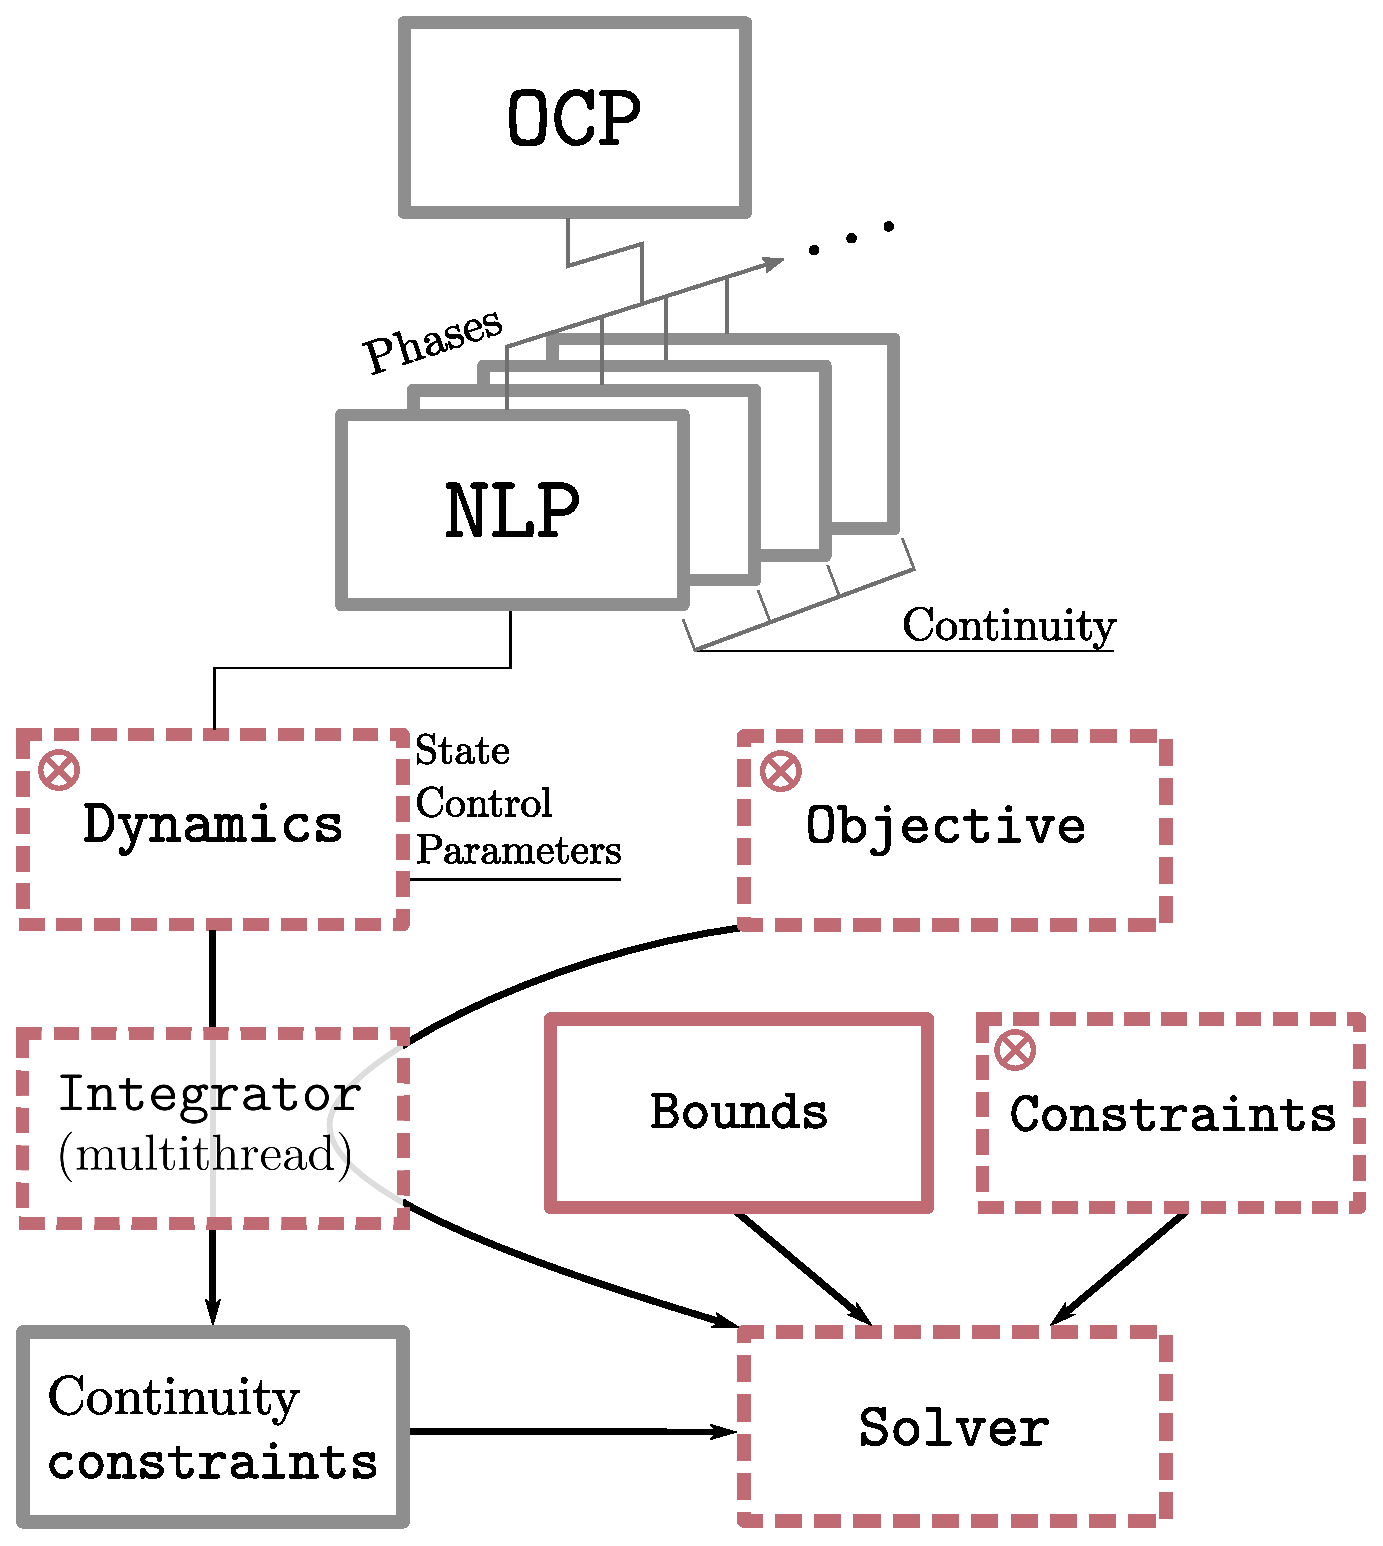
\includegraphics[width=0.9\columnwidth]{figures/design.eps}
\caption{\bioptim design flowchart.}
\label{fig:dependencies}
\vspace*{-0.5cm}
\end{figure}


\subsection{Design}
\bioptim shapes and solves optimal control problems whose two required entries are a model (.\textit{bioMod} file) and an OCP.
The model file contains the geometrical characteristics, the segment inertias, the geometrical markers, the actuators of the model (muscles and joint torques accounting for angle/angular velocity/torque relationships) as well as bounds on joint kinematics and torques. 
It also allows the user to design or import meshes for visualization purposes.
The OCP is implemented as a combination of nonlinear problems (NLPs) for allowing the formulation of multi-staged OCPs. Each NLP has the following attributes: a dynamics type, an objective function, constraints, a number of shooting points, the duration of the problem and initial guesses.
Based on these inputs, \bioptim properly sets up the multiple shooting transcription of the OCP, with appropriate continuity constraints in the case of multiple NLPs, and shapes it up to feed the chosen non-linear solver (Ipopt or Acados). 

\subsubsection{Dynamics types}
The dynamics type defines which variables are states ($\state$), which ones are controls ($\control$) and which ones are parameters ($\param$).
Then, it implements the ordinary differential equation governing the state transition:

\[
\dstate = f(\state, \control, \param).
\addtag
\label{eq:state_transition}
\]

\noindent More than 10 dynamics are implemented in \bioptim \footnote{\href{https://github.com/pyomeca/bioptim/blob/master/bioptim/dynamics/dynamics_functions.py}{github link}}, among which the controls can be muscle excitations/muscle activations/joint torques, the states can be joint kinematics/muscle activations, including/excluding contacts, etc.
Even if these dynamics types exhaustively span the current usages in biomechanics, a custom dynamics type is also pre-implemented to allow easy problem customization.

\subsubsection{Objective functions}
Accordingly to the optimal control formalism, there are two main types of objective functions, namely Lagrange and Mayer. Lagrange types are running objectives, integrated over the NLP duration. Mayer types are time-specific objectives. Classically, they correspond to a terminal objective, but to be more versatile, they can be defined at any instant in \bioptim.

These objective functions can depend on any of the optimization variable, \textit{i.e.} the controls, the states, the parameters and the duration of the problem. A lot of objective function types are already implemented in \bioptim ($>\!20$), among which tracking/minimizing, on the states/controls/markers/contact forces/problem duration, etc. Should one go missing, a custom objective type is also pre-implemented.

When declaring the desired list of objective function for a given NLP, each objective function type is associated with a weight, and the user can flexibly choose on which components of the vector variables the objective must apply. If applicable (for tracking objective functions mainly), the user must also specify the numerical target of the objective.

\subsubsection{Constraints}

\section{Examples}\label{sec:Examples}
\include{sections/Examples}

\section{Discussion}\label{sec:discussion}
The purpose of \bioptim is to solve a variety of biomechanical OCPs with minimal user effort and high performances in terms of computational time. 
The main features illustrated by the six provided examples are (Tab.~\ref{tab:Perfs_and_detailed_implementations_of_each_example}): 
\begin{itemize}
\item the possibility to use torque- or muscle-driven models (and their combinations);
\item a variety of ready-to-use cost functions, constraints and dynamics (with and without contacts)...
\item ... easily customizable in Python when required by the user;
\item the possibility to solve advanced OCPs (possibly multiphase) in a few seconds or minutes, that previously took us hours;
\item the interface with two different NLP solvers
\end{itemize}
In addition, every feature of \bioptim is thoroughly illustrated by the examples of the \href{https://github.com/pyomeca/bioptim/tree/master/examples/getting_started}{getting\_started} folder (parameter optimization, custom objects, etc.).
In the following, several aspects of \bioptim are discussed.


\subsection{Direct multiple shooting-based}

While the debate remains about the performances of direct collocations versus direct multiple shooting \cite{diehl2006fast, porsa2016direct}, the development of \bioptim was oriented toward the latter, because: \textit{i)} it allows to select effortlessly an arbitrary accuracy for the integration (e.g., order and numbers of RK steps); \textit{ii)} it allows to use multiple shooting-based fast NLP solvers such as \acados.
Concerning the integration, either internally or via \acados, several schemes are implemented in \bioptim (RK4, RK8, implicit RK).
While IRK showed better convergence in our experience with hard problems in \acados, RK4 showed to be a good speed/robustness tradeoff in most of the cases. 
In contrast to what is claimed in \cite{porsa2016direct}, direct multiple shooting is not a limitation to the performances (cost value and time to convergence), since, in our experience, the performances of \bioptim often outperform state-of-the-art results.

\subsection{Automatic differentiation}

One of the reasons explaining the performances of \bioptim is the rewriting of the core software, \textit{RBDL} \cite{felis2016rbdl} and \biorbd implementing the dynamics, into \casadi symbolics to automatically provide the exact Jacobians and Hessians of the resulting NLP.  
The gain in accuracy for the calculation of derivatives leads to shorter convergence times (due to much less iterations) and to optimal solutions reached with lower tolerances.
This last aspect must be emphasized for complex motions (fast, highly dynamics ones), because, for instance when using \ipopt, an optimal solution obtained with a convergence criterion of $10^{-2}$ is very unlikely to be dynamically sound; 
i.e., it would diverge when forwardly integrating the controls in a single-shooting manner. 
A lower tolerance ($10^{-6}$ or $10^{-8}$), which is only reachable with exact derivatives---for most of OCPs in biomechanics---, is expected to lead to better forward dynamics results.

\subsection{Python based, but fast!}

\bioptim was thought as an interface, and was therefore written in Python to allow the user to easily combine existing cost functions or constraints and self-implemented ones, to switch from one solver to another, etc. 
We believe this feature to be of importance given that the biomechanics community is mainly composed of software users rather than developers.
Therefore, providing a custom interface in Python rather than in C++, was a driving objective of our work to facilitate a rapid appropriation by the community.
Since flexibility and ease-of-use should not compromise the performances, the integration is multi-threaded and all the inside computations are expressed as C++ \casadi graphs, interfaced with C++ NLP solvers.
These graphs can either be built in \texttt{casadi.MX()} or \texttt{casadi.SX()}.
The latter requires more RAM for building the problem but is faster to solve.
While both may be used with \ipopt, \acados is only compatible with \texttt{casadi.SX()}.
By leveraging the speed of \texttt{casadi.SX()} graphs, we were able to estimate muscle forces in real time using \acados on a standard laptop (Ex.~\ref{ex:mhe}).
For a more in-depth analysis of the real-time estimation capabilities of \bioptim, see \cite{bailly2020real}.\\
Alongside with the 3D visualizer \bioviz that animates the solution, \bioptim proposes a series of online-generated figures, inspired by the  real-time graphics from \muscodii \cite{leineweber2003efficient1, leineweber2003efficient2}, to visualize the optimized variables at each iteration of the solver.
This is made with minimal computational cost thanks to the multiprocessing Python toolbox. 
Our implementation leverages the \textit{Python pickle} library for easily saving and loading OCPs for, e.g., post-processing analysis.
Finally, every layer (integration, optimization, visualization) of \bioptim is optimized to be flexible and fast.

\subsection{Fast vs robust NLP solvers}

Fast solvers, such as \acados, offer the opportunity to use multi-start approaches on complex problems, to circumvent the obstacle of local minima \cite{huchez2015local, bailly2020optimal}.
It also allows to get meaningful initial solutions from simpler problems, for guiding the resolution of the harder problems.
On the other hand, robust solvers, such as \ipopt, are convenient when the user lacks information about the sought solutions and thus cannot guide the solver through a good initial guess.
For biomechanics applications, the complementary characteristics of the interfaced solvers is a really useful tool.
Moreover, \bioptim's full compatibility with \casadi provides the opportunity to use any solver already interfaced with it, including third-party software such as \snopt, \textit{WORHP} \cite{wassel2013exploring} and \textit{KNITRO} \cite{nocedal2006knitro} (not tested yet). 

\subsection{Multiphase}

Biomechanics studies often face changing dynamics or objective functions due to the loss or gain of contacts or time-varying biomechanical tasks.
When tracking such a motion or trying to predict it, these changes translate into multiphase OCP.
This is one of the reported drawbacks of \moco, which does not provide this feature yet.
\bioptim, however, is able to handle multiphase OCPs, although they can currently only be solved with \ipopt (see Exs.~\ref{ex:walking} and \ref{ex:jump}).


\subsection{From constraints to objectives: easy problem relaxation}

As stated in Sec. II.B, there exists a correspondence between most of the pre-implemented \constraints and \objectives.
This is intended to allow for easy relaxation when the problem is reluctant to converge. 
For instance, when a biomechanical task requires the final configuration of the model to be enforced (reaching, cyclic motions, sports, etc.), one should first use a \constraint (e.g., \texttt{TRACK\_STATE}).
If the convergence is challenging, just turning this constraint into its namesake Mayer \objective, with a heavy weight, should help the solver.

\subsection{Limitations}

\bioptim is already a mature solution for solving biomechanical OCP. 
However some limitations should be raised. 
First, it is based on  \biorbd which is not as advanced as \opensim or \anybody (AnyBody Technology) in terms of biomechanical features and audience.
Nevertheless,  \biorbd is actively maintained, fast and \casadi-compatible for automatic differentiation.
The variety of proposed examples highlighted simple to advanced models.
Even if defining a new model was made straightforward thanks to the \texttt{.bioMod} file format, \textit{biorbd} does not include a GUI for building models. 
Some Opensim models can be translated into \texttt{.bioMod} but \biorbd does not yet support multiple wrapping objects, non-orthogonal DoFs between bodies, compliant contact force models (\cite{serrancoli2019subject}) or muscle-tendon equilibrium. 
As seen in \cite{dembia2020opensim}, wrapping objects are rare due to the computational cost and required optimization when a line of action is in contact with more than one object, which compromises automatic differentiation. 
Via-points and pre-processed moment arms \cite{van2011implicit} (to be expressed as polynomial functions of crossed DoFs) are often preferred. 

\subsection{Future directions}

\bioptim, code name \textit{PaperWork} (Version 1.1.0), was released in February 2021, with all the features presented in this communication.
Some improvements are expected in a near future.
First, a graphical model builder is planned in \biorbd, to easily generate \textit{.bioMod} files.
Also, models of muscular fatigue are to be included in \bioptim, to predict adapted motor strategies for long or demanding motions.
The formulation of moving horizon schemes (MHE, Nonlinear Model Predictive Control) will be pre-implemented, with efficient warm-starting heuristics, to facilitate their use.
The implementation of muscle-tendon equilibrium is planned for fast movements or those with large ranges of motions. 
It will require an additional optimization step to achieve the equilibrium as done in \textit{CEINMS} \cite{pizzolato2015ceinms} or the addition of muscle lengths as state variables, as in \cite{van2011implicit}.  
Moreover, an effort will be made to extend the compatibility of \acados with all the features of \bioptim (multiphase, nonlinear constraints, etc.). 
Finally, we plan to add an inverse optimal control module to \bioptim and muscle synergy dynamics to improve motion predictions \cite{walter2014muscle}.


\section*{Acknowledgment}
This study and the biorbdp library development was partly funded by scholarships of the  Vanier program (BM) and the TransMedTech Institute XXX Apogée Canada (FB) and MB NSERC Discovey Programme (XXXX). Biorbdoptim acts as a catalyst in our group and several students contribute to this library; thank you to Amedeo, Ariane, André, Kilperic. 





\bibliographystyle{IEEEtran}
\bibliography{biblio}

\newpage
\appendix
The appendix\label{sec:appendix}

\end{document}
